\documentclass[ngerman]{dis-template-add}


\renewcommand{\Aufgabenblatt}{4}
\renewcommand{\Ausgabedatum}{19. Mai 2020}
\renewcommand{\Abgabedatum}{09. Juni 2020}
\renewcommand{\Gruppe}{Simon Weidmann, Aram Yesildeniz}
\renewcommand{\STiNEGruppe}{14}


\begin{document}


\section*{Report}

\subsection*{a)}
There is a singleton PersistenceManager.
He holds atomic Integers for LSN and TID values, so that there are no duplicates for those.

Then he also holds two hashtables.
One is for the buffer, mapping pageIDs to buffer pages.
BufferPage is a data type that holds TID, pageID, LSN and data (string).
The second one is for the transactions (this one could easily be implemented with simple lists as well), mapping TIDs to booleans, saying true if the transaction is committed, falso otherwise.

On beginTransaction(), a new TID is polled and a new entry is inserted into the transaction hashtable.

On commit(TID), a new LSN ist polled, an EOT is logged (new log entry) and the transaction hashtable entry for that TID is set to true.

On write(TID, pageID, data), a new LSN is polled, a new BufferPage is created that holds all information (see above) and a corresponding log entry is written.
If the buffer now exceed the threshhold, committed transactions will be persisted.
This is simply done by iterating over the transaction hashtable to find out which transactions are commited.
Then we iterate over the buffer and persist the committed transactions.

\medskip

There is one RecoveryTool instantiated by the PersistenceManager.
It iterates over the log, chooses winner TAs by finding the EOT strings in the log.
Then it iterates over the log again and for the winner TAs checks if the log entry has a higher LSN than the actual persisted data page.
If not, the logged data will be persisted.


\subsection*{b)}
\subsubsection*{i)}

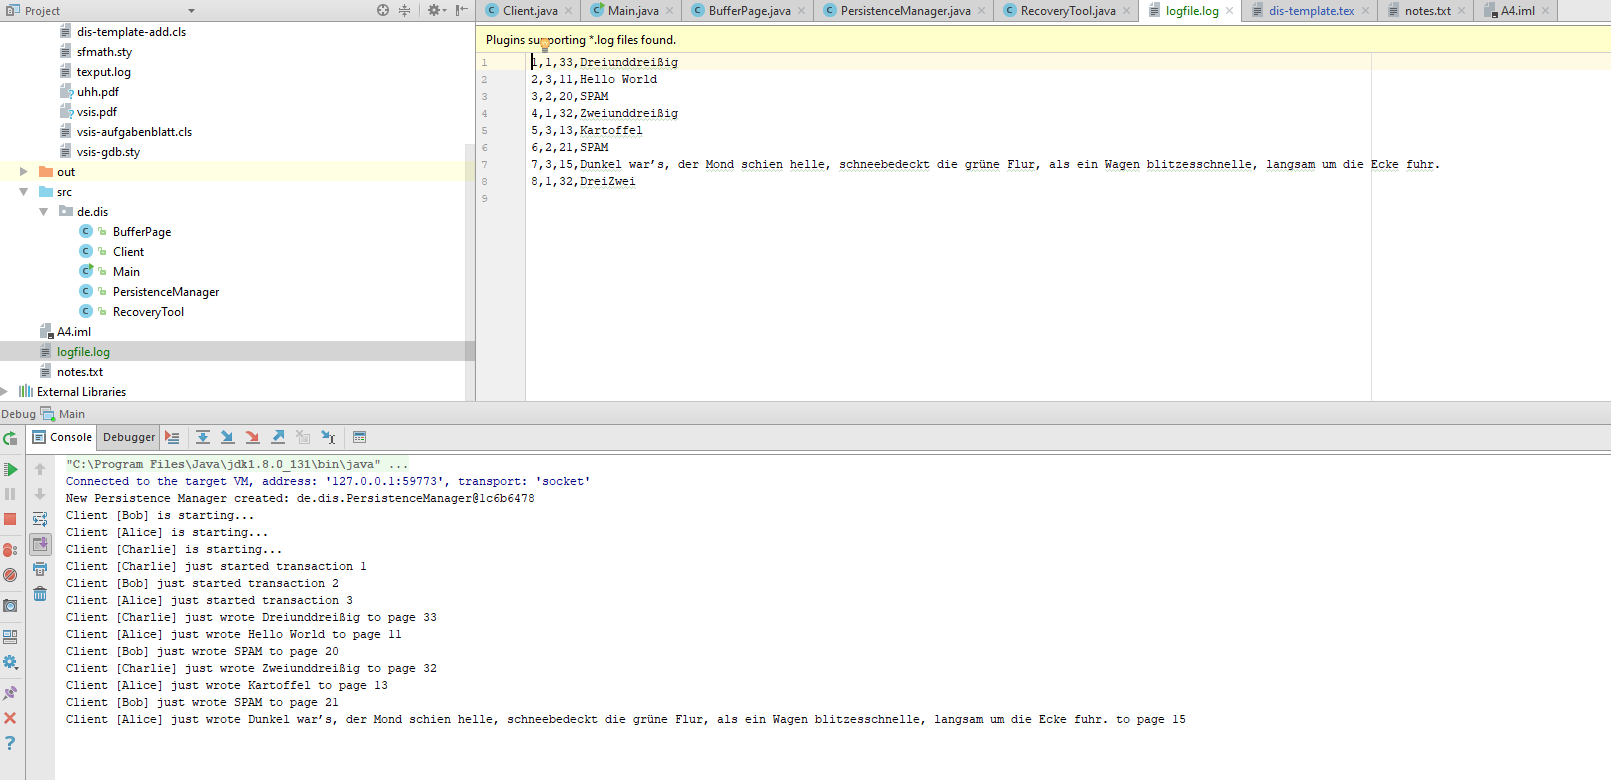
\includegraphics[scale=0.4]{exb.png}

As you can see, there are several log entries but no files written (on the left, should be in same directory as the logfile.log)

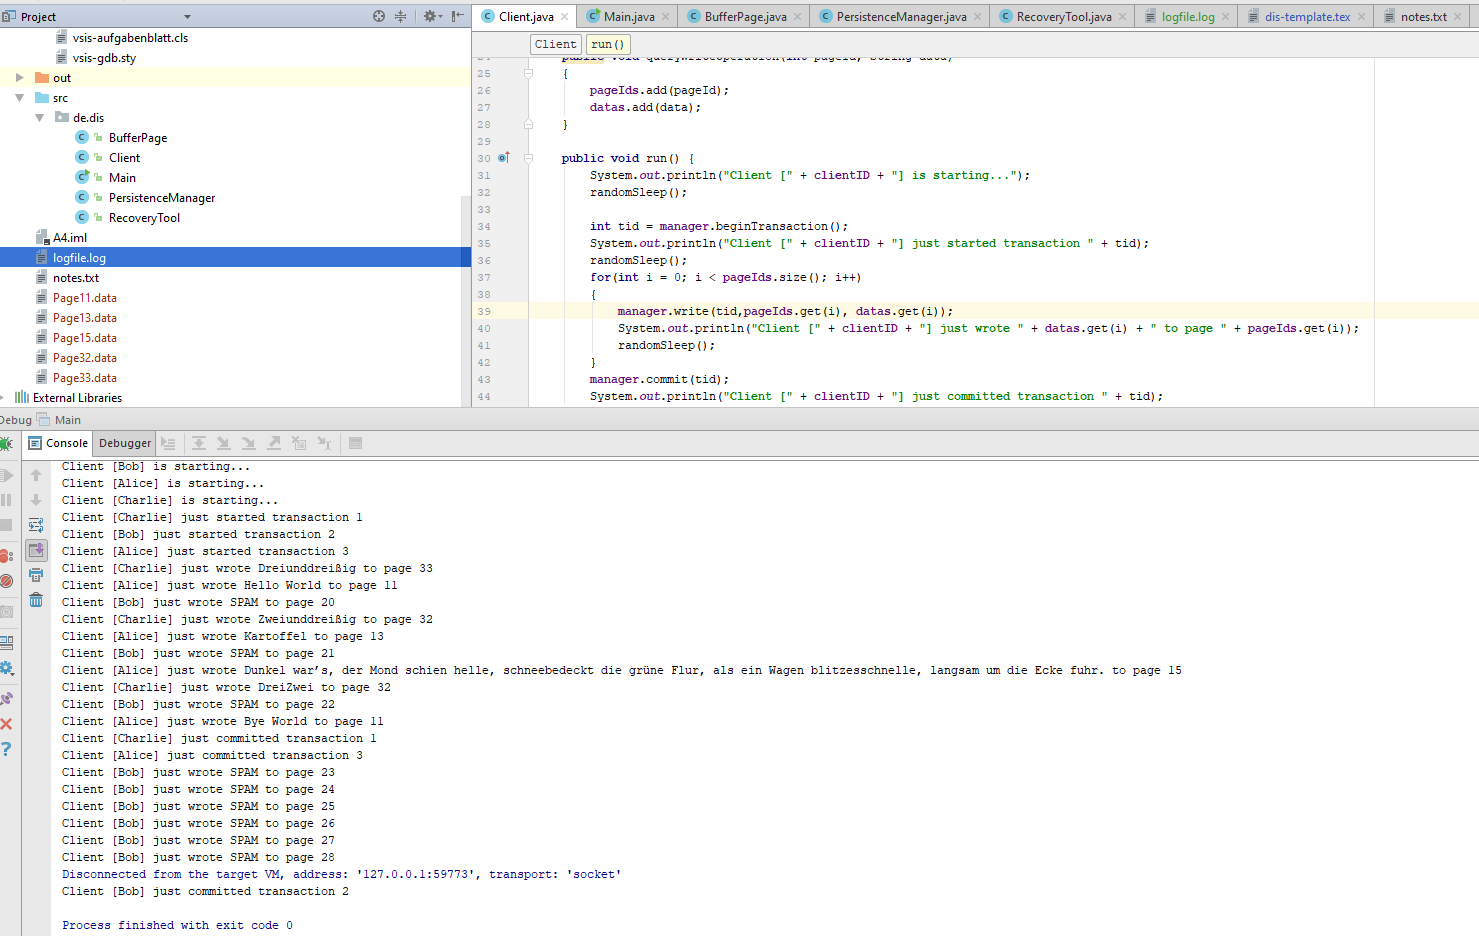
\includegraphics[scale=0.4]{exb2.png}

This is what it looks like after all the commits. Some of the pages are still not persisted as described in the excercise.
You could easily implement this to persist all before closing the application.

\subsection*{c)}
\subsubsection*{i)}
We delete the page 11:

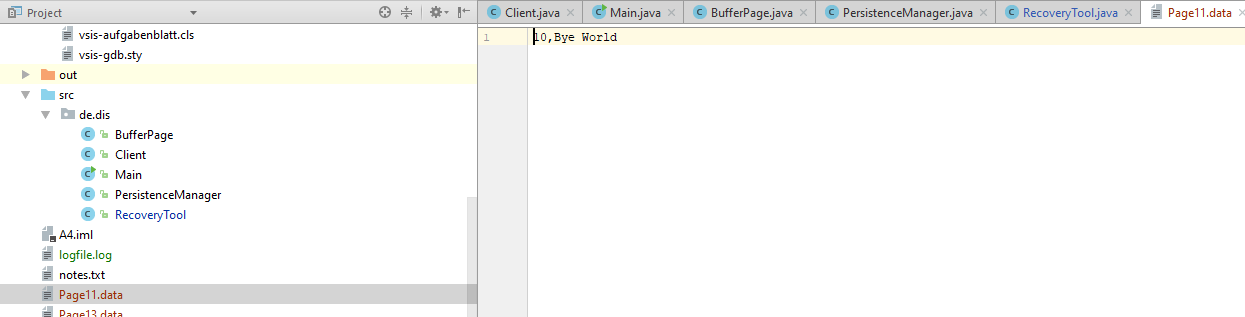
\includegraphics[scale=0.5]{excp11.png}

We modify page 32 by adding some stuff in Capslock:

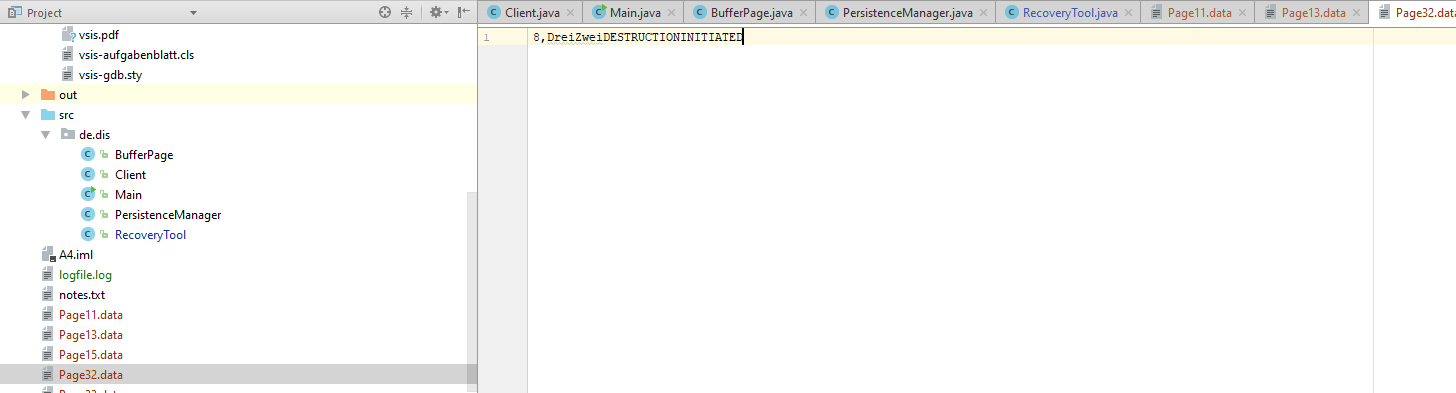
\includegraphics[scale=0.5]{excp32.png}

After the recovery, page 11 is restored and the page 32 modification is reverted (note that some other pages were recovered, those that have not been persisted yet after the last run. That was just because Client Alices (pages in the 20s) was the last to commit its transaction and no further write operation was performed afterwards):

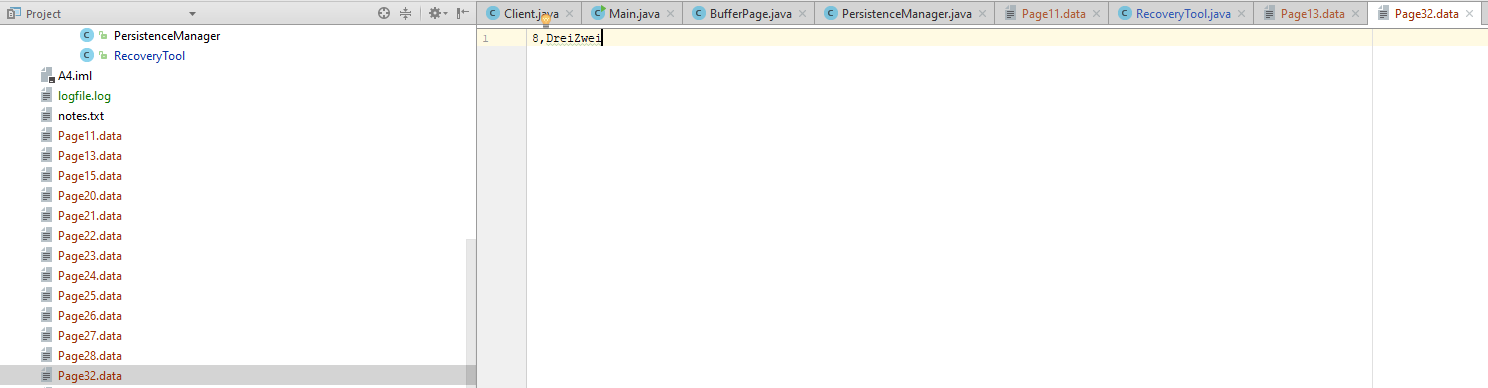
\includegraphics[scale=0.5]{excrecovered.png}

The exact behavior on the restoration depends on if you actively restore from log entries with LSN that are $\geq$ than the persisted one or only greater than them.
For both cases, an argument can be made
In our case, it does the $\geq$.
The lecture says to do it the other way. it would not do a restore.
It might do a full consistency check as we will describe below in c)iii), which is very easy to implement (if wanted).

\subsubsection*{ii)}
We have already seen in the last excercise, that Alice's transaction is not persisted after her commit, as the persisting is only triggered by write() operations.
So her pages are not even existing yet when the program closes the first time (see in c)i)).
As her transaction is fully logged, it is recovered at the next recovery step (see above as well.)

\subsubsection*{iii)}
Nothing happens. Therefore we omit the screenshot.
There is no mechanism that would find in error in the data when seeing a higher LSN.
One could implement a consistency check in all the data pages, checking if their data is actually the one that it should be according to the log file.
The algorithm would go through all pages, check their LSN and look back into the log file if the data is logged as it is persisted.
We were not sure if this was intended by looking into the lecture slides.
The implementation would be a simple for loop over the log winners and looking into the individual pages.

\end{document}